\documentclass[aspectratio=169,12pt]{beamer}
\usepackage{amsmath}
\usepackage{amssymb}
\usepackage{array}
\usepackage[most]{tcolorbox}
\usepackage{graphicx}
\usepackage{tikz}
\usepackage[sfdefault,lf]{FiraSans}
\renewcommand{\familydefault}{\sfdefault}
\setlength{\parindent}{0pt}
\everymath{\displaystyle}

\setbeamertemplate{navigation symbols}{}
\setbeamertemplate{footline}{}
\setbeamertemplate{headline}{}
\setbeamertemplate{blocks}[rounded][shadow=false]

\definecolor{mmpageWhite}{HTML}{FCFBF7}
\definecolor{mmtanSoft}{HTML}{F7F5EF}
\definecolor{mmgreenDeep}{HTML}{244B2C}
\definecolor{mmgreenLeaf}{HTML}{5D8A56}
\definecolor{mmgreenSoft}{HTML}{E4EFD9}
\definecolor{mmtext}{HTML}{163221}
\definecolor{mmwarn}{HTML}{8F2F36}
\definecolor{mmwarnSoft}{HTML}{F8E8EA}

\setbeamercolor{background canvas}{bg=mmpageWhite}
\setbeamercolor{normal text}{fg=mmtext,bg=mmpageWhite}
\setbeamercolor{block title}{fg=mmgreenDeep,bg=mmgreenSoft}
\setbeamercolor{block body}{fg=mmtext,bg=mmtanSoft}
\setbeamercolor{block title example}{fg=mmgreenDeep,bg=mmgreenSoft}
\setbeamercolor{block body example}{fg=mmtext,bg=white}
\setbeamercolor{block title alerted}{fg=mmwarn,bg=mmwarnSoft}
\setbeamercolor{block body alerted}{fg=mmtext,bg=white}
\setbeamercolor{itemize item}{fg=mmgreenDeep}
\setbeamercolor{itemize subitem}{fg=mmgreenDeep}

\newtcolorbox{MMCard}[2][]{enhanced,breakable=false,colback=#2,colframe=black,boxrule=1.5pt,arc=8pt,left=5pt,right=5pt,top=4pt,bottom=4pt,before skip=0pt,after skip=0pt,#1}
\newcommand{\KoruIcon}{\raisebox{-0.2em}{\includegraphics[height=1.05em]{../../../manamaths/SITE/header-logo.png}}}
\newcommand{\NotesTitle}[1]{{\colorbox{mmtanSoft}{\parbox{0.975\linewidth}{\vspace{0.14em}\hspace{0.25em}{\LARGE\bfseries\textcolor{mmgreenDeep}{#1}\hfill\KoruIcon}\vspace{0.14em}}}\par\vspace{0.18em}{\color{mmgreenLeaf}\rule{\linewidth}{2.0pt}}\par\vspace{0.12em}}}
\newcommand{\SectionTitle}[1]{{\large\bfseries\textcolor{mmgreenDeep}{#1}}\par\vspace{0.04em}}
\newcommand{\GreenDivider}{\par\vspace{0.01em}{\color{mmgreenLeaf}\rule{\linewidth}{2.4pt}}\par\vspace{0.03em}}
\newcommand{\KeyIdea}[1]{\begin{MMCard}[title={\textbf{Key idea}},colbacktitle=mmgreenSoft,coltitle=mmgreenDeep]{mmtanSoft}\small #1\end{MMCard}}
\newcommand{\WorkedExample}[2]{\begin{MMCard}[title={\textbf{#1}},colbacktitle=mmgreenSoft,coltitle=mmgreenDeep]{white}\small #2\end{MMCard}}
\newcommand{\CommonMistake}[1]{\begin{MMCard}[title={\textbf{Common mistake}},colbacktitle=mmwarnSoft,coltitle=mmwarn]{white}\small #1\end{MMCard}}
\newcommand{\TryThese}[1]{\begin{MMCard}[title={\textbf{Try these}},colbacktitle=mmgreenSoft,coltitle=mmgreenDeep]{mmtanSoft}\small #1\end{MMCard}}
\newcommand{\StepLine}[2]{\textbf{#1.} #2\par\vspace{0.03em}}

\setbeamertemplate{background}{
 \begin{tikzpicture}[remember picture,overlay]
 \draw[black,line width=1.5pt,rounded corners=10pt]
 ([xshift=0.45cm,yshift=-0.45cm]current page.north west)
 rectangle
 ([xshift=-0.45cm,yshift=0.45cm]current page.south east);
 \end{tikzpicture}
}

\begin{document}

\begin{frame}[t,shrink=8]
\NotesTitle{Nets of 3D shapes}

\begin{columns}[T,onlytextwidth]
\begin{column}{0.48\textwidth}
\KeyIdea{A net is a flat 2D shape that folds to form a 3D shape. Different 3D shapes have different nets. Some shapes, like cylinders, have curved surfaces that flatten to rectangles.}
\SectionTitle{Steps for identifying a net}
\StepLine{1}{Identify the 3D shape the net represents.}
\StepLine{2}{Count the faces and check they match the shape.}
\StepLine{3}{Visualise folding along the edges.}
\StepLine{4}{Check that opposite faces are in the right positions.}

\CommonMistake{Thinking a cylinder has no net. A cylinder has a curved surface that unfolds to a rectangle, plus two circles.}
\end{column}
\begin{column}{0.48\textwidth}
\WorkedExample{Cylinder net}{A cylinder net has three parts:
\begin{itemize}
\item Two circles (top and bottom faces)
\item One rectangle (curved surface unfolded)
\end{itemize}
The width of the rectangle equals the circumference of the circle ($2\pi r$). The height of the rectangle is the height of the cylinder.

\begin{center}
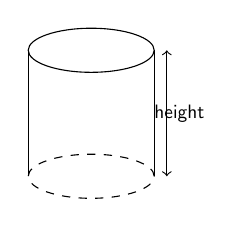
\begin{tikzpicture}[x=0.4cm,y=0.4cm]
\draw[dashed] (0,0) ellipse (2 and 0.7);
\draw (0,4) ellipse (2 and 0.7);
\draw (-2,0) -- (-2,4);
\draw (2,0) -- (2,4);
\node[scale=0.7] at (2.8,2) {height};
\draw[<->] (2.4,0) -- (2.4,4);
\end{tikzpicture}
\end{center}
}
\end{column}
\end{columns}
\GreenDivider
\TryThese{
\begin{enumerate}
\item How many faces does a cylinder have?
\item Name the shapes that make up a cylinder's net.
\item A cylinder has height 6 cm and radius 2 cm. What is the width of the rectangle in its net?
\end{enumerate}
}
\end{frame}

\end{document}
